\documentclass{standalone}
\usepackage{tikz}

\newcommand{\bt}{\mathbf{t}}
\newcommand{\bx}{\mathbf{x}}
\newcommand{\by}{\mathbf{y}}
\newcommand{\bz}{\mathbf{z}}
\newcommand{\eq}{=}




\begin{document}
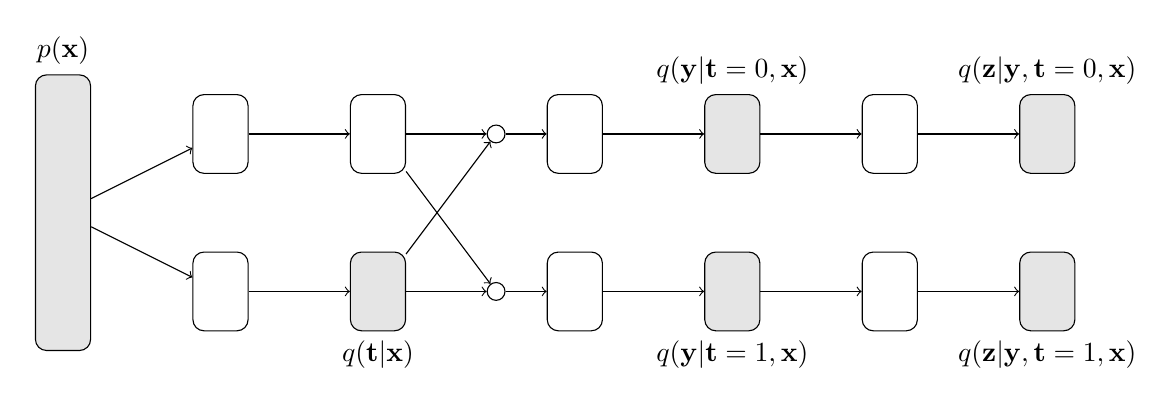
\begin{tikzpicture}
    \node[draw, minimum width=0.7cm, minimum height=3.5cm, rounded corners, label=$p(\bx)$, fill=black!10!white] (x) at (0, 0) {};
    \node[draw, minimum width=0.7cm, minimum height=1cm, rounded corners] (x1) at (2, 1) {};
    \node[draw, minimum width=0.7cm, minimum height=1cm, rounded corners] (x2) at (2, -1) {};
    \node[draw, minimum width=0.7cm, minimum height=1cm, rounded corners] (x11) at (4, 1) {};
    \node[draw, minimum width=0.7cm, minimum height=1cm, rounded corners, label=below:$q(\bt|\bx)$,fill=black!10!white] (qt) at (4, -1) {};
    
    \node[draw, circle, inner sep=0.08cm] (switch1) at (5.5, 1) {};
    \node[draw, circle, inner sep=0.08cm] (switch2) at (5.5, -1) {};
    
    \node[draw, minimum width=0.7cm, minimum height=1cm, rounded corners] (x13) at (6.5, 1) {};
    \node[draw, minimum width=0.7cm, minimum height=1cm, rounded corners] (x23) at (6.5, -1) {};
    \node[draw, minimum width=0.7cm, minimum height=1cm, rounded corners, label={$q(\by|\bt \eq 0, \bx)$}, fill=black!10!white] (qyt0) at (8.5, 1) {};
    \node[draw, minimum width=0.7cm, minimum height=1cm, rounded corners, label=below:{$q(\by | \bt=1,\bx)$}, fill=black!10!white] (qyt1) at (8.5, -1) {};
    
    \node[draw, minimum width=0.7cm, minimum height=1cm, rounded corners] (x14) at (10.5, 1) {};
    \node[draw, minimum width=0.7cm, minimum height=1cm, rounded corners] (x24) at (10.5, -1) {};
    \node[draw, minimum width=0.7cm, minimum height=1cm, rounded corners, label={$q(\bz | \by,\bt \eq 0, \bx)$}, fill=black!10!white] (qzt0) at (12.5, 1) {};
    \node[draw, minimum width=0.7cm, minimum height=1cm, rounded corners, label=below:{$q(\bz | \by, \bt=1,\bx)$}, fill=black!10!white] (qzt1) at (12.5, -1) {};


    \draw[->] (x) to (x1);
    \draw[->] (x) to (x2);
    \draw[->] (x1) to (x11);
    \draw[->] (x2) to (qt);
    \draw[->] (qt) to (switch1);
    \draw[->] (qt) to (switch2);
    \draw[->] (x11) to (switch1);
    \draw[->] (x11) to (switch2);
    
    \draw[->] (switch1) to (x13);
    \draw[->] (x13) to (qyt0);
    \draw[->] (qyt0) to (x14);
    \draw[->] (x14) to (qzt0);
    
    \draw[->] (switch2) to (x23);
    \draw[->] (x23) to (qyt1);
    \draw[->] (qyt1) to (x24);
    \draw[->] (x24) to (qzt1);
\end{tikzpicture}
\end{document}